%
% File emnlp2018.tex
%
%% Based on the style files for EMNLP 2018, which were
%% Based on the style files for ACL 2018, which were
%% Based on the style files for ACL-2015, with some improvements
%%  taken from the NAACL-2016 style
%% Based on the style files for ACL-2014, which were, in turn,
%% based on ACL-2013, ACL-2012, ACL-2011, ACL-2010, ACL-IJCNLP-2009,
%% EACL-2009, IJCNLP-2008...
%% Based on the style files for EACL 2006 by
%%e.agirre@ehu.es or Sergi.Balari@uab.es
%% and that of ACL 08 by Joakim Nivre and Noah Smith

\documentclass[11pt,a4paper]{article}
\usepackage[hyperref]{emnlp2018}
\usepackage{times}
\usepackage{latexsym}
\usepackage{url}
\usepackage{amsmath}
\usepackage{algorithm}
\usepackage{algorithmic}
%%% YOUR PACKAGES BELOW THIS LINE %%%
\usepackage[small,bf]{caption} % added MLF 20171211
\usepackage{multicol}
\usepackage{adjustbox}
\usepackage{graphicx}
\usepackage{array,multirow}

\aclfinalcopy % Uncomment this line for the final submission

\setlength\titlebox{5cm}
% You can expand the titlebox if you need extra space
% to show all the authors. Please do not make the titlebox
% smaller than 5cm (the original size); we will check this
% in the camera-ready version and ask you to change it back.

\newcommand\BibTeX{B{\sc ib}\TeX}
\newcommand\confname{EMNLP 2018}
\newcommand\conforg{SIGDAT}

\title{Fixing Translation Divergences in Parallel Corpora for Neural MT}
%\title{A Recurrent Network for Parallel Corpora Divergence Analysis}

\author{MinhQuang Pham$^{\dag\ddag}$, \ \ Josep Crego$^\dag$,\ \ Jean Senellart$^\dag$ ,\ \ Fran\c cois Yvon$^\ddag$\\
  $^\dag$SYSTRAN / 5 rue Feydeau, 75002 Paris, France\\
  {\tt firstname.lastname@systrangroup.com}\\
  $^\ddag$LIMSI, CNRS,  Universit\'e Paris-Saclay 91405 Orsay, France\\
  {\tt firstname.lastname@limsi.fr}} 

\date{}

\begin{document}
\maketitle

\begin{abstract}
%http://www.airccj.org/CSCP/vol4/csit42503.pdf

Corpus-based approaches to machine translation rely on the availability of clean parallel corpora.
%In the case of neural machine translation, a large neural network is trained to maximise the translation performance on a given parallel corpus. 
Such resources are scarce, and because of the automatic processes involved in their preparation, they are often noisy. % may contain sentence pairs that are not as parallel as one would expect.
This paper describes an unsupervised method for detecting translation divergences in parallel sentences. We rely on a neural network that computes cross-lingual sentence similarity scores, which are then used to effectively filter out divergent translations. Furthermore, similarity scores predicted by the network are used to identify and fix some partial divergences, yielding additional parallel segments. We evaluate these methods for English-French and English-German machine translation tasks,  and show that using filtered/corrected corpora actually improves MT performance.

\end{abstract}

\section{Introduction}

Parallel sentence pairs are the only necessary resource to build Machine Translation (MT) systems. 
In the case of neural MT, a large neural network is trained through maximising a proxy of translation performance on a parallel corpus. 
Therefore, the quality of MT engines is heavily dependent on the amount but also the quality of available parallel sentences.\footnote{Recent work on neural MT~\cite{lample2018word,artetxe2018iclr} completely dispenses with parallel data, using unsupervised methods to obtain performance improvements over word-by-word statistical MT. These systems however lag far behind supervised systems, as considered in this work.} 

Parallel texts are unfortunately, scarce resources:
There are relatively few language pairs for which parallel corpora of large sizes exist, and even for those pairs, available corpora only concern few restricted domains. 
To alleviate the lack of parallel data, several approaches have been developed over the years. 
They range from methods using non-parallel, or comparable data 
~\cite{Zhao:2002:APS:844380.844785,W04-3208,J05-4003,GregoireL18,P17-3003,P18-2037} to techniques that produce synthetic parallel data from monolingual corpora ~\cite{P16-1009,W17-4714}, using automated alignment/translation engines that are prone to the introduction of noise in the resulting parallel sentences. 
Mismatches in parallel sentences extracted from translated texts are also reported ~\cite{tiedemann2011bitext,XU16.310}. 
This problem is mostly ignored in MT, where parallel sentences are considered to convey the exact same meaning; yet it seems particularly important for neural MT engines~\cite{chen2016adaptation}.

\begin{table}[ht]
\small
\center
\begin{tabular}{ c|l }
  \hline  
  \texttt{en} & \it{What do you feel}\bf{, Spock}\it{?} \\
  \texttt{fr} & \it{Que ressentez-vous?} \\
  \texttt{gl} & {\small \it{What do you feel?}} \\
  \hline
  \texttt{en} & \it{How much do you get paid?} \\
  \texttt{fr} & \it{T'es pay\'e combien} \bf{de l'heure}\it{?} \\
  \texttt{gl} & {\small \it{How much do you get paid per hour?}} \\
  \hline  
  \texttt{en} &  \bf{That seems a lot.} \\
  \texttt{fr} & \bf{40 livres?} \\
  \texttt{gl} & {\small \it{40 pounds?}} \\
  \hline  
  \texttt{en} & \it{I brought you} \bf{french fries}\it{!} \\
  \texttt{fr} & \it{Je t'ai rapport\'e des} \bf{saucisses}\it{!} \\
  \texttt{gl} & {\small \it{I brought you sausage!}} \\
  \hline
\end{tabular}
\caption[Table caption text]{Examples of semantically divergent parallel sentences. English (\texttt{en}), French (\texttt{fr}) and gloss of French (\texttt{gl}). Divergences are in bold letters. }
\label{tab:examples}
\end{table}

Table~\ref{tab:examples} gives some examples of English-French parallel sentences that are not completely semantically equivalent, extracted from the OpenSubtitles corpus ~\cite{LisonTiedemann2016}. 

Multiples types of translation divergences are found in parallel corpora:
Additional segments are included on either side of the parallel sentences (first and second rows) most likely due to errors in sentence segmentation;
Some translations may be completely uncorrelated (third row);
Inaccurate translations also exist (fourth row). 
Note that divergent translations can be due various reasons~\cite{C14-1055}, the study of which is beyond the scope of this paper. 

In this work, we present an unsupervised method for building cross-lingual sentence embeddings based on modelling word similarity,  % in the form of continuous vectors. 
relying on a neural architecture (see \textsection~\ref{sec:divergence}) that is able to identify several types of common cross-lingual divergences. 
% which are common to many existing bi-texts.
The resulting embeddings are then used to measure semantic equivalence between sentences.
To evaluate our method, we show in \textsection~\ref{experiments} that translation accuracy can be improved after filtering out divergent sentence pairs in an English-to-French and an English-to-German translation tasks.
We also show that in some cases, divergent sentences can be fixed by removing divergent segments, further increasing translation quality. All the code used in this paper is freely available.\footnote{https://github.com/jmcrego/similarity}

% Useless for a short
% The remainder of this paper is structured as follows. 
% Section~\ref{related} overviews related work. 
% We describe in detail the core of the neural divergence classifier in Section. 
% We report experiments with the presented model in Section
% Section~\ref{sec:results} evaluates results. 
% Finally, conclusions are drawn in Section~\ref{conclusions} and further work is outlined in Section~\ref{further}.

\section{Related Work}
\label{related}

Attempts to measure the impact of translation divergences in MT have focused on the introduction of noise in sentence alignments~\cite{goute2012}, showing that statistical MT is highly robust to noise, and that performance only degrades seriously at very high noise levels.  In contrast, neural MTs seem to be more sensitive to noise~\cite{chen2016adaptation}, as they tend to assign high probabilities to rare events~\cite{Hassan2018AchievingHP}.

Efforts devoted to characterising the degree of semantic equivalence between two snippets of texts in the same or different languages are presented~\cite{conf/semeval/AgirreBCDGMRW16}. % a workshop devoted to an objective similar to our work. 
In~\cite{Mueller:2016:SRA:3016100.3016291}, a monolingual sentence similarity network is proposed, making use of a simple LSTM layer to compute sentence representations. 
The authors show that a simple SVM classifier exploiting such sentence representations achieves state-of-the-art results in a textual entailment task. 
With the same objective, the system of~\citet{N16-1108} uses multiple convolutional layers and models pairwise word interactions. %Our work differs from the previous as we build a different network and use it to measure similarity of sentences in different languages. 

Our work is inspired by~\citet{W17-3209}, who train a SVM-based cross-lingual divergence detector using word alignments and sentence length features. 
Their work shows that an NMT system trained only on non-divergent sentences yields slightly better translation scores, while requiring less training time. 
A follow-up study by the same authors~\cite{N18-1136} achieves even better results, using the neural architecture of \citet{N16-1108}.
Our work differs from theirs as we make use of a network with a different, arguably simpler, topology. 
We model sentence similarity by means of optimising a loss function based on word alignments. 
Furthermore, the network predicts word similarity scores that we further use to correct divergent sentences.

\section{Neural Divergence Classifier}
\label{sec:divergence}

The architecture of our network is inspired by the work on word alignment of~\citet{W16-2207}, using however contextual, rather than fixed, word embeddings (see Figure~\ref{network}).
\begin{figure}[h]
\center
    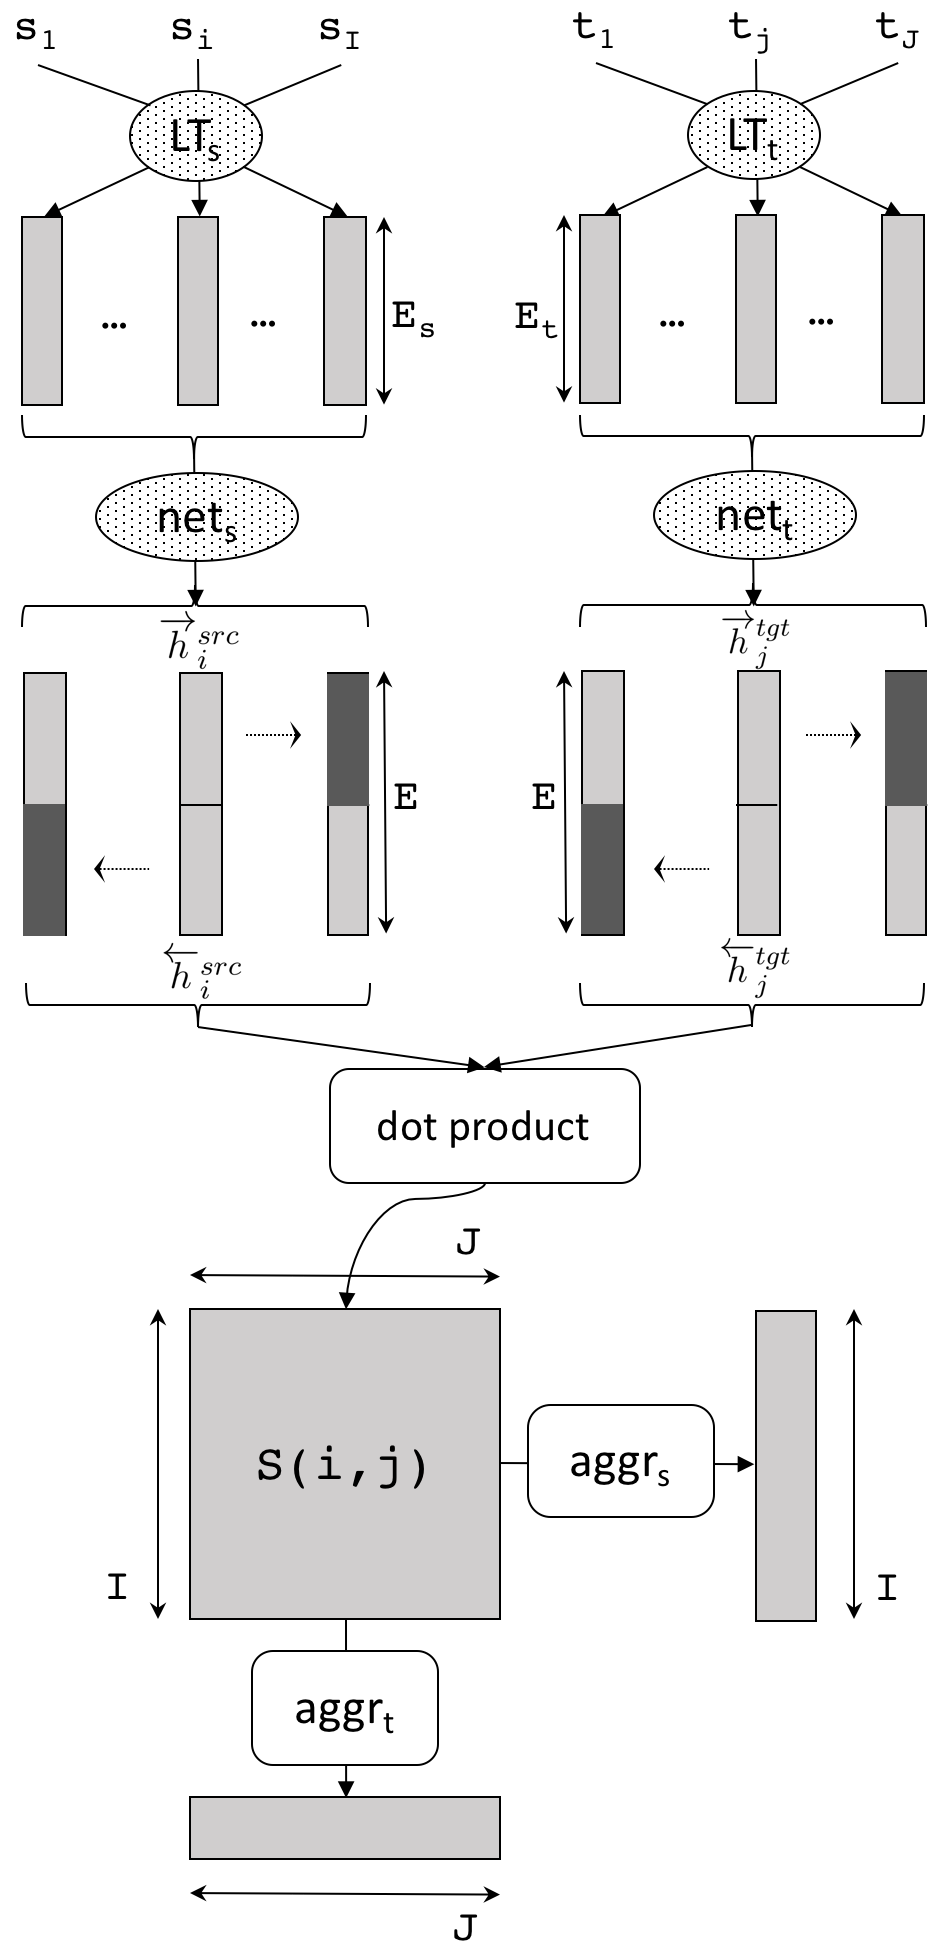
\includegraphics[width=0.8\linewidth]{network}
    \caption{Illustration of the model.} 
    \label{network}
\end{figure}
 
%\subsection{Divergence Network}

It computes the similarity of any source-target sentence pair $(s,t)$, where $s=(s_1,...,s_I)$ and $t=(t_1,...,t_J)$. 
The model is composed of 2~bi-directional LSTM subnetworks, $net_s$ and $net_t$, which respectively encode source and target sentences. 
Since both $net_s$ and $net_t$ take the same form, we only describe the former network: 
it outputs forward and backward hidden states, $\overrightarrow{h}^{src}_i$ and $\overleftarrow{h}^{src}_i$, which are then concatenated into a vector encoding the $i^{th}$ source word as $h^{src}_i = [ \overrightarrow{h}^{src}_i ; \overleftarrow{h}^{src}_i ]$.
In addition, the last forward/backward hidden states (in dark grey on Figure~\ref{network}) are also concatenated  to represent whole sentences 
$h_{src} = [ \overrightarrow{h}^{src}_I ; \overleftarrow{h}^{src}_1 ]$.
The similarity between sentence pairs can then be obtained using eg.\ the cosine similarity:
\begin{equation}
    sim(h_{src}, h_{tgt}) = \frac{h_{src} \cdotp h_{tgt}}{||h_{src}|| * ||h_{tgt}||}
    \label{cosine}
\end{equation}
%\noindent where two vectors (embeddings) with the same orientation have a cosine similarity of $1$, while two vectors with opposed orientation have a similarity of $-1$, independent of their magnitude.

Our model is trained to maximize word alignment scores between words in both sentences, using aggregation functions that summarise the alignment scores for each source/target word. 
Similar to~\cite{W16-2207}, alignment scores $S(i,j)$ are given by the dot-product $S(i,j) = h_i^{src} \cdotp h_j^{tgt}$, further aggregated as follows:
\begin{equation}
\begin{split}
    aggr_s(i,S) = \frac{1}{r} \ log \left( \displaystyle \sum_{j=1}^{J} e^{r * S(i,j)}\right) \\
    aggr_t(j,S) = \frac{1}{r} \ log \left( \displaystyle \sum_{i=1}^{I} e^{r * S(i,j)}\right)
\end{split}
\label{aggregation}
\end{equation}


The training loss function is then defined as:
%\vspace{-8mm}
\begin{equation}
\begin{split}
\mathcal{L}(src,tgt) = \ \ \ \ & \\
    \sum_{i=1}^I log(1+e&^{aggr_s(i,S) * sign_i}) \ \ +\\
 + \sum_{j=1}^J log(1+e&^{aggr_t(j,S) * sign_j})
\end{split}
\label{loss_wemb}
\end{equation}
%\vspace{-8mm}

\subsection{Training with Negative Examples}
\label{negative}

Training is performed by minimizing Eq.~\eqref{loss_wemb}, for which annotated examples of source ($\operatorname{sign}_i$) and target ($\operatorname{sign_j}$) words are needed.
As positive examples, we use paired sentences of a parallel corpus; all words in such sentences are labelled as parallel ($ \forall i, j, \operatorname{sign}_i=\operatorname{sign}_j=-1$). %, $sign_i=-1$ and $sign_j=-1$. 
We consider three types of negative instances: the basic case uses random unpaired sentences; in this case, all words are labelled as divergent ($ \forall i, j, \operatorname{sign}_i=\operatorname{sign}_j=+1.$). %, $sign_i=+1$ and $sign_j=+1$. 
Since negative pairs may be very easy to classify and we want our network to detect less obvious divergences, we further create more difficult negative examples as follows.

We first replace random sequences of words in source or target by a sequence of words with the same part-of-speeches.\footnote{The rationale is to try to keep the generated sentences as grammatical as possible; 
Otherwise, the network could learn to flag non-grammatical sentences as non-parallel.}
 Words that are not replaced are deemed parallel ($\operatorname{sign}_i=-1$) while those replaced are annotated as $\operatorname{sign}_i=+1$. 
Words aligned to some replaced words are also assigned the divergent label ($\operatorname{sign}_i=+1$). For instance, given the original sentence pair:

\begin{table}[h]
\center
\begin{tabular}{ll}
src: & { \small \texttt{What do you feel ?}} \\
tgt: & { \small \texttt{Que ressentez-vous ?}} \\
\end{tabular},
\end{table}

\noindent we may replace '\texttt{you feel}', with part-of-speech tags '\texttt{PRP VB}', by another sequence with same tags (i.e. '\texttt{we want}'), yielding a new negative instance (divergent words are in bold):  
\begin{table}[h]
\center
\begin{tabular}{ll}
src: & { \small \texttt{What do {\bf we \ want} ?}} \\
$\mathcal{Y}^{src}$: & { \small \texttt{-1 \ \  -1 {\bf +1\ \ +1} \ \  -1}} \\
tgt: & { \small \texttt{Que {\bf ressentez-vous} ?}} \\
$\mathcal{Y}^{tgt}$: & { \small \texttt{-1\ \ {\bf +1}\ \ \ \ \ \ \ \ \ -1}} \\
\end{tabular}
\end{table}

% Note that the new sentences are not assured to be grammatical after replacing sequences with the same part-of-speech.
Note that we need word alignments to identify as divergent the sequence '\texttt{ressentez-vous}', which was aligned to '\texttt{you feel}' in the original sentence.
Finally, motivated by sentence segmentation errors observed in many corpora, we also build negative examples by inserting a sentence at the beginning (or end) of the source (or target) sentence. 
Words in the original sentence pair are annotated $\operatorname{sign}_i=-1$, while the new words inserted are considered divergent ($\operatorname{sign}_i=+1$).
Given the same sentence pair as above, a negative example is created by inserting the sentence '\texttt{Not .}' at the end of the original source:

\begin{table}[h]
\center
\begin{tabular}{ll}
src: & { \small \texttt{What do you want ? {\bf Not \ .}}} \\
$\mathcal{Y}^{src}$: & { \small \texttt{-1 \ \  -1 -1 \ -1  \ \ -1 {\bf +1\ \ \  +1}}} \\
tgt: & { \small \texttt{Que ressentez-vous ?}} \\
$\mathcal{Y}^{tgt}$: & { \small \texttt{-1\ \ -1\ \ \ \ \ \ \ \ \ \ \ \ \ -1}} \\
\end{tabular}
\end{table}

% Replace and insert methods are applied on either side of the sentence pairs. 
To finally avoid the generation of easy negative sentence pairs having a large difference in sentence length, we restrict negative examples to have a length ratio $< 2.0$ ($3.0$ for shortest sentences).

\subsection{Divergence Correction}
\label{correction}

Our training corpora contains many divergent sentences that follow a common pattern, consisting of adding some extra leading/trailing words. % (as in the first and second examples of table~\ref{tab:examples}). 
Accordingly, we implemented a simple algorithm that discards sequences of leading/trailing words on both sides. 
% Hence considering as parallel $s_u^v$ and $t_x^y$. 
To find optimal source ($u, v$) and target ($x, y$) indices that enclose parallel segments within the original sentence, we compute:
\begin{equation*}
\underset{u, v, x, y}{\arg\max} \Big \{      \underset{u \le I \le v}{\sum} \underset{x \le j \le y}{\max} \{ S(i,j) \}    \Big \}
\end{equation*}
The $\mathcal{N}$-best sequences ($s_u^v$, $t_x^y$) are considered as likely corrections, in which we select the one having the highest sentence-level similarity to replace the original $(s_1^I, t_1^J)$.
Note that short sentences are not considered and we enforce $v - u > \tau$ and $y - x > \tau $. 
Figure~\ref{matrix} (left) displays an example of an alignment matrix $S(i,j)$.
An acceptable correction is: \textit{Que ressentez-vous ? $\Leftrightarrow$ What do you feel ?}. 
corresponding to $u=1$, $v=5$, $x=1$ and $y=3$.

\section{Experiments}
\label{experiments}

%In this section we report on the experiments conducted to evaluate the proposed methods. %We begin with details of the corpora employed.

\subsection{Corpora}
\label{corpora}

We filter out divergences from the English-French OpenSubtitles corpus~\cite{LisonTiedemann2016}, which consists of a collection of movie and TV subtitles. 
We also use the very noisy English-German Paracrawl\footnote{http://paracrawl.eu/} corpus. Both corpora present many potential divergences.
To evaluate English-French translation performance, we use the En-Fr Microsoft Spoken Language Translation corpus, created from actual Skype conversations~\cite{mslt-corpus-iwslt-2016-release}. 
English-German performance is evaluated on the publicly available Newstest-2017~\cite{W17-4717}, corresponding to news stories selected from online sources.

In order to better assess the quality of our classifier when facing different word divergences, we also collected from the original OpenSubtitles corpus $500$ sentences containing different types of examples:
$200$ paired sentences;
$100$ unpaired sentences;
$100$ sentences with replace examples; and
$100$ sentences with insert examples (see \textsection~\ref{negative}).
All data is preprocessed with \texttt{OpenNMT}\footnote{http://opennmt.net}, performing minimal tokenisation. %, basically splitting-off punctuation.
After tokenisation, each out-of-vocabulary word is mapped to a special UNK token, assuming a vocabulary containing the $50,000$ more frequent words.

\subsection{Neural Divergence}
\label{divergence}

Word embeddings of $E_s=E_t=256$ cells are initialised using \texttt{fastText},\footnote{https://github.com/facebookresearch/fastText} further aligned by means of \texttt{MUSE}\footnote{https://github.com/facebookresearch/MUSE} following the unsupervised method of~\citet{lample2018word}. Both bi-LSTMs use $256$-dimensional hidden representations ($E=512$).
Network optimization is done using SGD with gradient clipping~\cite{Pascanu:2013:DTR:3042817.3043083}. 
For each epoch, we randomly select $1$ million sentence pairs that we place in batches of $32$ examples.  
We run $10$ epochs and start decaying at each epoch by $0.8$ when the loss on validation set increases. 
Divergence is computed as in equation~\eqref{cosine} and setting $r=1.0$ ; 
For divergence correction, we use $\mathcal{N}=20$ and $\tau=3$.
The same number of examples are always generated for each type of example ({\texttt P}aired, {\texttt U}npaired, {\texttt R}eplace and {\texttt I}nsert). 
Alignments needed for {\texttt R}eplace and {\texttt I}nsert methods are performed using \texttt{fast\_align}\footnote{https://github.com/clab/fast\_align}.

\subsection{Neural Translation}
\label{translation}

In addition to the basic tokenisation detailed above, we perform Byte-Pair Encoding~\cite{Sennrich2016} with $30000$ merge operations learned by joining both language sides.
Neural systems are based on the open-source project  \texttt{OpenNMT};  using a Transformer model similar to the model of~\citet{vaswani2017attention}: both encoder and decoder have $6$ layers; Multi-head attention is performed over $8$ head;
the hidden layer size is $512$; and the inner layer of feed forward network is of size $2048$. 
Word embeddings have $512$ cells. We set the dropout probability to $0.1$ and the batch size to $3072$.
%The maximum length of both source and target sentences is set to $80$ and we limit the vocabulary size to $50,000$ words for both source and target languages. 
The optimiser is Lazy Adam with $\beta_1 = 0.9$, $\beta_2 = 0.98$, $\epsilon = 10^{-9}$, $warmup\_steps = 4000$. Training stops after $30$ epochs.

\section{Results}
\label{sec:results}

We first evaluate the ability of our divergence classifier to predict different types of divergences at the level of words. 
We use the test set manually annotated for that purpose and train our model on the OpenSubtitles corpus.
A word is considered divergent when associated to a negative aggregation score (see Equation~\eqref{aggregation}).
Accuracies obtained for various combinations of negative examples, where we see that
non-divergent words in parallel and unpaired sentences (columns \texttt{P} and \texttt{U}) are easy to spot, as long as the model has seen these types of examples in training. 
However, the accuracy drops dramatically when the model is not trained with unpaired sentences (rows  \texttt{PR}, \texttt{PI} and \texttt{PRI}).
Regarding columns \texttt{R} and \texttt{I}, accuracies are lower since these sentences contain a mix of divergent and non-divergent words. 

\begin{table}[h]
\small
\center
\begin{tabular}{crccccc}
\hline
\multicolumn{2}{l}{\bf Accuracy} & \multicolumn{5}{c}{Test examples} \\
 &  & \texttt{P} & \texttt{U} & \texttt{R} & \texttt{I} & \texttt{PURI} \\
 \hline
\parbox[t]{0mm}{\multirow{7}{*}{\rotatebox[origin=c]{90}{Train examples}}} &  \texttt{PU}     & \bf 0.996 & \bf 0.994 & 0.671 & 0.673 & 0.874 \\
 &  \texttt{PR}     & \bf 0.995 &      0.033 & \bf 0.951 &      0.689 & 0.746 \\
 &  \texttt{PI}       & \bf 0.998 &      0.071 &      0.697 & \bf 0.725 & 0.705 \\
 &  \texttt{PUR}  & \bf 0.994 & \bf 0.989 & \bf 0.919 &      0.710 & 0.932 \\
 &  \texttt{PUI}    & \bf 0.995 & \bf 0.996 &      0.662 & \bf 0.769 & 0.887 \\
 &  \texttt{PRI}    & \bf 0.991 &      0.161 & \bf 0.924 & \bf 0.719 & 0.768 \\
 &  \texttt{PURI} & \bf 0.995 & \bf 0.980 & \bf 0.916 & \bf 0.788 & \bf 0.942 \\
\hline
\end{tabular}
\caption{Word divergence accuracies according to different type of examples used in train/test.}
\label{results_puri}
\end{table}

Models that were trained with the matching examples (\texttt{R} and \texttt{I}) obtain the highest accuracies (in bold letters).
Column \texttt{PURI} gives results for the complete test set, mixing all type of examples. 
As expected, the best accuracy is also obtained when training on all types of  examples. 

Figure~\ref{matrix} illustrates the output of our network when trained using \texttt{PU} examples (right) and \texttt{PURI} examples (left).  
The former (right) fails to predict some divergences, most likely because its training set does not contain sentences mixing divergent and non-divergent words. 
Furthermore, the network trained with \texttt{PURI} examples correctly assigns a lower similarity score to this pair, as both sentences do not convey the exact same meaning.


%\vspace{-3mm}
\begin{figure}[h]
\centering
    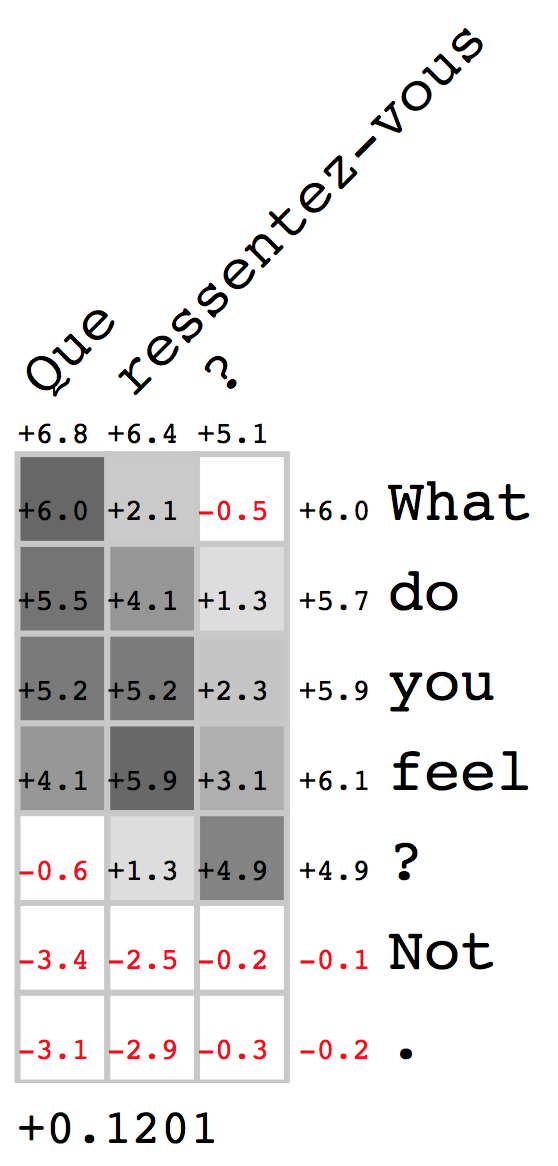
\includegraphics[width=0.35\linewidth]{feel}    
    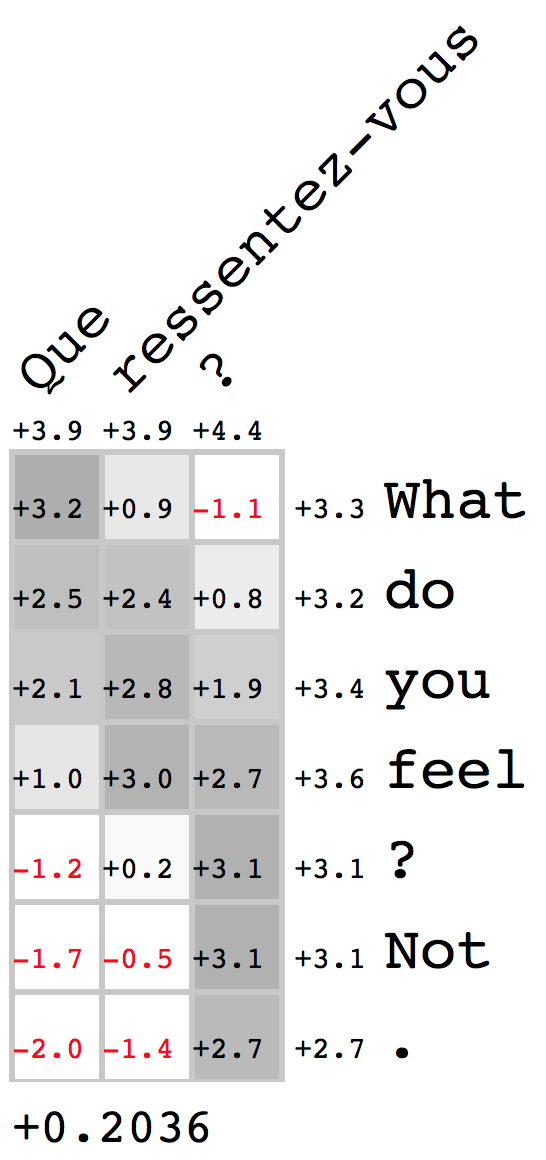
\includegraphics[width=0.35\linewidth]{feel_pu}    
\caption{Sentence pair with similarity scores produced by our model when trained with \texttt{PU} examples (right) and over \texttt{PURI} examples (left). Aggregation scores (Eq.~\eqref{aggregation}) are shown next to words. Matrices contain alignment scores. Sentence similarities (Eq.~\eqref{cosine}) are below matrices.}
\label{matrix}
\end{figure}

Finally, BLEU scores obtained with varying training data configurations are in Table~\ref{results}:
The entire\footnote{Paracrawl contains more than $100$M sentences. We reduced its size to $22.2$M using standard filtering techniques.} data sets (\texttt{all}); 
The most similar pairs after optimizing Eq.~\eqref{loss_wemb} (\texttt{sim}); 
After applying the correction algorithm of \textsection~\ref{correction} (\texttt{sim+fix}).
Columns Ref and Fix indicate the number of original and corrected sentences (in millions) used in training.

\begin{table}[h!]
\small
\center
\begin{tabular}{lccl}
\hline
\bf Data & \bf Ref (M) & \bf Fix (M) & \bf Test (BLEU) \\ %MSLT & \bf NEWS \\
\hline
\multicolumn{3}{c}{\scriptsize{OpenSubtitles English-French}} \\
\texttt{all}                   & 27.2 & - & 42.18 \\
%\texttt{semb}             & 18.0 & - & \\
\texttt{sim}            & 15.5 & - & 43.12  ($+0.94$)\\
%\texttt{sim}           & 21.5 & - & 42.56 \\
\texttt{sim}           & 18.0 & - & 43.19  ($+1.01$)\\
\texttt{sim+fix}     & 15.5 & 2.5 & \bf 44.19 ($+2.01$)\\
%\texttt{sim+fix}   & 15.5 & 5.0 & \\
\hline
\multicolumn{3}{c}{\scriptsize{Paracrawl English-German}} \\
%\texttt{all}                  & 100.0 & 12.56 \\ 
\texttt{all}                  & 22.2 & - & 19.27 \\ 
%\texttt{semb}            & 15.0 & - & \\
\texttt{sim}           & 15.0 & - & 21.52 ($+2.25$)\\
\texttt{sim}           & 17.5 & - & 21.97 ($+2.70$)\\
\texttt{sim+fix}   & 15.0 & 2.5 & \bf 22.42 ($+3.15$) \\
\hline
\end{tabular}
\caption{BLEU scores obtained by neural MT using different subsets of the OpenSubtitles and Paracrawl corpora.}
\label{results}
\end{table}

Results obtained after filtering sentence pairs (\texttt{sim}) clearly outperform the baseline (\texttt{all}) by $+0.94$ and $+2.25$ BLEU respectively.
Regarding OpenSubtitles, when fixing $2.5$M sentences ($4^{th}$ row) the accuracy is further boosted to $+2.01$, whereas the same sentence pairs do not show any improvement when added in their original form ($3^{rd}$ row).
Similar results are obtained for the Paracrawl corpus. Results after fixing $2.5$M sentences ($4^{th} row$) outperform those obtained with their original form ($3^{rd} row$).


\section{Conclusions and outlook}
\label{conclusions+further}

We presented an unsupervised method based on deep neural networks for detecting translation divergences in parallel corpora. 
Our model optimizes word alignments, and computes a fine grained divergence prediction at the level of words. 
Misaligned/divergent words can then be filtered out, yielding larger and better training sets. 
Our experiments on two machine translation tasks show significant improvements in comparison to training with the entire data set. 
%The method can be used on any parallel corpus without any manual annotation.

%We plan to further evaluate divergence classification under different data noise levels. %and on additional language pairs. 
%as well as to measure the impact of using less noisy data when learning the similarity model
%We also would like to evaluate the impact of using less noisy (already filtered) data to learn the similarity model. 
%We would also like to use our model to predict other types of divergences 
We plan to use our model to predict sentence embeddings over monolingual corpora, allowing to collect parallel pairs through vector similarity measures.
%We also plan to further evaluate the correction algorithm.
In addition, we would like to measure the performance of our model after applying subword tokenisation,
%when working with a reduced vocabulary set, as a result of applying any subword tokenisation,
as well as using multiple LSTM layers, a technique well known to capture hierarchical structure in the context of MT.

\section*{Acknowledgements}
We are grateful to J. Legrand for his fruitful comments regarding the neural divergence classifier.

\bibliography{biblio}
\bibliographystyle{acl_natbib_nourl}

\end{document}
